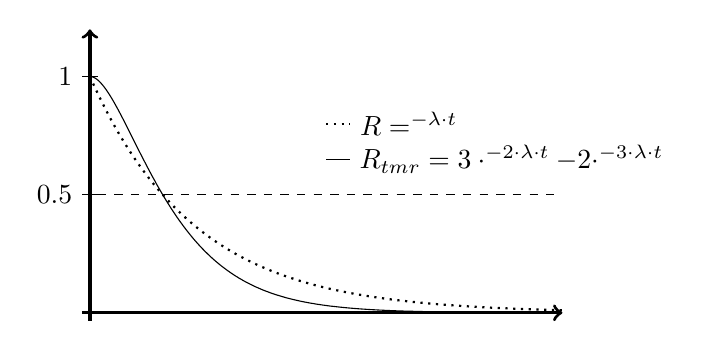
\begin{tikzpicture}[yscale=3]
\def\dtx{0.1}
\def\dty{0.1}
\def\dx{6}
\def\la{0.75}
\draw[->,very thick] (0,-0.0333) -- (0,1.2);
\draw[->,very thick] (-0.1,0) -- (\dx,0);
\foreach \y in {0.5,1} {
  \draw (\dtx,\y) -- (-\dtx,\y) node[anchor=east]{$\y$};
}
\draw[dashed,thin] (\dtx,0.5) -- (\dx,0.5);
\draw[dotted,thick] plot[domain=0:6,samples=400] (\x,{exp(-\la*\x)});
\draw plot[domain=0:6,samples=400] (\x,{3*exp(-2*\la*\x)-2*exp(-3*\la*\x)});
\draw[dotted,thick] (3,0.8) -- ++(0.3,0) node[anchor=west] {$R=\conse^{-\lambda\cdot t}$};
\draw (3,0.65) -- ++(0.3,0) node[anchor=west] {$R_{tmr}=3\cdot\conse^{-2\cdot\lambda\cdot t}-2\cdot\conse^{-3\cdot\lambda\cdot t}$};
\end{tikzpicture}